% =============================================================================
\section{Cómo están hechos los mundos}
% =============================================================================

\begin{frame}{Un mundo = un .sdf generado}
  \begin{columns}[c]
    \column{0.5\textwidth}
    \begin{tikzpicture}[node distance=0.5cm,every node/.style={font=\scriptsize}]
      \node[draw=azul,fill=azulclaro,rounded corners,minimum width=3.4cm] (b) {tools/build\_worlds.py};
      \node[draw,rounded corners,below left=0.6cm and -1.2cm of b,minimum width=2.2cm,align=center] (m) {models/x500\_mallas\\(.obj con UVs)};
      \node[draw,rounded corners,below right=0.6cm and -1.2cm of b,minimum width=2.2cm,align=center] (w) {worlds/<mundo>/\\<mundo>.sdf + spawn.yaml};
      \node[draw,rounded corners,below=1.9cm of b,minimum width=3.4cm,align=center] (f) {models/: Fuel + texturas\\(copiados, sin internet)};
      \draw[-{Stealth}] (b) -- (m); \draw[-{Stealth}] (b) -- (w);
      \draw[-{Stealth},dashed] (f) -- (w);
    \end{tikzpicture}
    \column{0.47\textwidth}\small
    \begin{itemize}
      \item \cmd{python3 tools/build\_worlds.py} reescribe \textbf{todos} los mundos.
      \item Cambiar un mundo = cambiar el script y regenerar. Cambios a mano en el
        \cmd{.sdf} se pierden.
      \item Luego \cmd{vespo build} para instalarlos.
    \end{itemize}
  \end{columns}
\end{frame}

\begin{frame}{Las piezas}
  \begin{columns}[t]
    \column{0.32\textwidth}
    \begin{idea}[title={\small\bfseries Modelos de Fuel},coltitle=black,colbacktitle=azulclaro]
      \scriptsize Casas, árboles, coches, postes, fuente, bancas, camión, rocas (OpenRobotics,
      CC0 / CC BY). Copiados en \cmd{models/}.
    \end{idea}
    \column{0.32\textwidth}
    \begin{idea}[title={\small\bfseries Texturas},coltitle=black,colbacktitle=azulclaro]
      \scriptsize De ambientCG (CC0): pasto, adoquín, concreto, calle, roca, madera, ladrillo, grava.
      Color + normal + rugosidad (PBR).
    \end{idea}
    \column{0.32\textwidth}
    \begin{idea}[title={\small\bfseries Lo propio},coltitle=black,colbacktitle=azulclaro]
      \scriptsize Piso, puente, farmacia, cueva, bodegas, balizas, geocerca, estación: cajas,
      cilindros y mallas que escribe el script.
    \end{idea}
  \end{columns}
  \vspace{0.5em}
  \small Licencias y lista completa en \cmd{CREDITS.md}.
\end{frame}

\begin{frame}{¿Por qué mallas y no un \texttt{<plane>}?}
  \begin{columns}[c]
    \column{0.5\textwidth}\small
    Un \cmd{<plane>} de Gazebo estira \textbf{una} imagen sobre todo su tamaño: una textura de
    pasto de 1 m sobre 260 m se ve borrosa.
    \vspace{0.3em}

    El script escribe mallas \cmd{.obj} cuyas coordenadas UV son \emph{metros / tamaño del mosaico}:
    la textura se repite cada 2--4 m.
    \column{0.47\textwidth}
    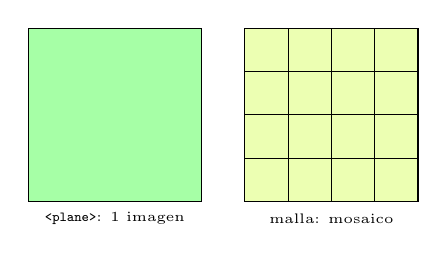
\begin{tikzpicture}[scale=0.55]
      \draw[fill=green!35] (0,0) rectangle (4,4);
      \node[font=\tiny] at (2,-0.4) {\texttt{<plane>}: 1 imagen};
      \begin{scope}[xshift=5cm]
        \foreach \i in {0,1,2,3} \foreach \j in {0,1,2,3} \draw[fill=green!25!yellow!30] (\i,\j) rectangle (\i+1,\j+1);
        \node[font=\tiny] at (2,-0.4) {malla: mosaico};
      \end{scope}
    \end{tikzpicture}
  \end{columns}
\end{frame}

\begin{frame}{Colisiones: siempre cajas}
  \small
  \begin{itemize}
    \item El motor de física de Gazebo (dartsim) no choca de forma confiable contra \textbf{mallas}.
    \item Por eso lo propio lleva \textbf{cajas y cilindros} como colisión, aunque se vea con malla:
      el puente, las paredes de la cueva (una caja cada \textasciitilde1 m), las bodegas, la cerca.
    \item Las paredes rojas de la geocerca y los haces de las balizas son \textbf{solo visuales}:
      el dron las atraviesa.
  \end{itemize}
  \begin{ojo}
    \small Si agregan un obstáculo, agreguen su \cmd{collision()} además del \cmd{visual()}.
    Si solo se ve, el dron lo atraviesa; si solo choca, el lidar o la cámara no lo ven.
  \end{ojo}
\end{frame}

\begin{frame}[fragile]{Agregar algo a un mundo}
  \begin{lstlisting}[style=cpp,language=Python,caption={Dentro de build\_plaza\_show(), por ejemplo}]
# Un poste de 3 m en (5, -5) de Gazebo, que se ve y choca:
stage.solid(cyl(0.2, 3.0), tex('concreto_claro'), pose(5, -5, 1.5))

# Un modelo de Fuel (ya copiado en models/):
extras.append(include('oak_tree', 'arbol_extra', 12, 3))

# Una luz:
lights.append(point_light('foco', 0, 10, 3.0, (1.0, 0.8, 0.5), rng=12))
  \end{lstlisting}
  \begin{lstlisting}[style=bash,caption={Regenerar, revisar e instalar}]
python3 src/x500_retos/tools/build_worlds.py
gz sdf -k src/x500_retos/worlds/plaza_show/plaza_show.sdf    # "Valid."
vespo build
  \end{lstlisting}
\end{frame}

\begin{frame}{Lecciones (1/3): lo que rompía el render}
  \small
  \begin{enumerate}
    \item \textbf{Texturas con el mismo nombre}: ogre2 identifica una textura por el nombre del
      archivo, no por la carpeta. \cmd{pasto/color.jpg} y \cmd{madera/color.jpg} salían iguales.
      Solución: nombres únicos (\cmd{pasto\_color.jpg}).
    \item \textbf{Casas negras}: los modelos viejos de Fuel usan scripts de material de Ogre 1, que
      Gazebo Harmonic ignora. Se cambiaron por materiales PBR con las mismas texturas.
    \item \textbf{Personas caminando} (\cmd{<actor>}): congelaban el render de la cámara. No hay
      actores en los mundos.
  \end{enumerate}
\end{frame}

\begin{frame}{Lecciones (2/3): lo que hacía lenta la simulación}
  \begin{columns}[c]
    \column{0.55\textwidth}\small
    El puente corría a \textbf{0.27$\times$} tiempo real. La causa: una roca y un camión de Fuel que
    \textbf{no eran estáticos}. La roca pesa 2.5 t y tiene colisión de malla: la física la
    calculaba chocando contra el terreno a cada paso.
    \vspace{0.3em}

    Con \cmd{<static>true</static>} el mundo regresó a \textbf{1.0$\times$}.
    \column{0.42\textwidth}
    \begin{idea}
      \small Todo lo que es decorado va \textbf{estático}. Lo único que se mueve en nuestros
      mundos es el dron y la camioneta sospechosa.
    \end{idea}
  \end{columns}
\end{frame}

\begin{frame}{Lecciones (3/3): la cámara que llenó la RAM}
  \begin{columns}[c]
    \column{0.55\textwidth}\small
    PX4 carga en todos los mundos el plugin \cmd{GstCameraSystem}: toma la primera cámara y la manda
    como video H.264 por UDP.
    \begin{itemize}
      \item Sin CUDA codifica por software y no alcanza.
      \item Su cola (\cmd{appsrc}) no tiene límite: guarda \textbf{todas} las imágenes.
      \item Gazebo llegó a \textbf{13.4 GB} y la computadora se trabó.
    \end{itemize}
    \column{0.42\textwidth}
    \begin{idea}
      \small Los mundos con cámara (\cmd{zona\_bodegas}, \cmd{base\_carga}) declaran sus sistemas
      a mano, sin ese plugin (\cmd{CAMERA\_WORLD\_SYSTEMS}). Con eso Gazebo se queda en
      \textasciitilde820 MB.
    \end{idea}
  \end{columns}
\end{frame}

\begin{frame}{El modelo x500\_cam\_abajo}
  \begin{columns}[c]
    \column{0.5\textwidth}\small
    \begin{itemize}
      \item El x500 de PX4 + una cámara hacia abajo, 10 cm bajo el centro.
      \item 960\,$\times$\,720 a 15 Hz (\textasciitilde31 MB/s), campo de visión de 1.74 rad
        (100°), igual que la de PX4.
      \item Su airframe \cmd{4501\_gz\_x500\_cam\_abajo} vive junto al modelo; \cmd{vespo
        simulate} lo enlaza al build de PX4.
    \end{itemize}
    \column{0.47\textwidth}
    \begin{tikzpicture}[scale=0.9]
      \draw[thick,fill=gray!20] (-1,0) rectangle (1,0.3);
      \fill (0,-0.05) rectangle (0.2,-0.15);
      \draw[azul,dashed] (0.1,-0.15) -- (-1.8,-2.6);
      \draw[azul,dashed] (0.1,-0.15) -- (2.0,-2.6);
      \draw[thick] (-2.4,-2.6) -- (2.6,-2.6);
      \node[font=\tiny] at (0.1,-2.85) {a 15 m ve \textasciitilde36 m de ancho};
      \node[font=\tiny,azul] at (1.6,-1.2) {100°};
    \end{tikzpicture}
  \end{columns}
\end{frame}

\begin{frame}{Lo que solo existe en simulación}
  \begin{columns}[c]
    \column{0.55\textwidth}\small
    \textbf{La camioneta sospechosa se mueve sola}: el plugin \cmd{VelocityControl} de Gazebo le da
    velocidad constante (3 m/s) y giro constante ($\omega = v/R$), así que da vueltas a un círculo
    de 26.5 m de radio sin que ningún nodo le mande nada.
    \[ R = \frac{v}{\omega} = \frac{3}{0.1132} = 26.5\ \text{m} \]
    \column{0.42\textwidth}
    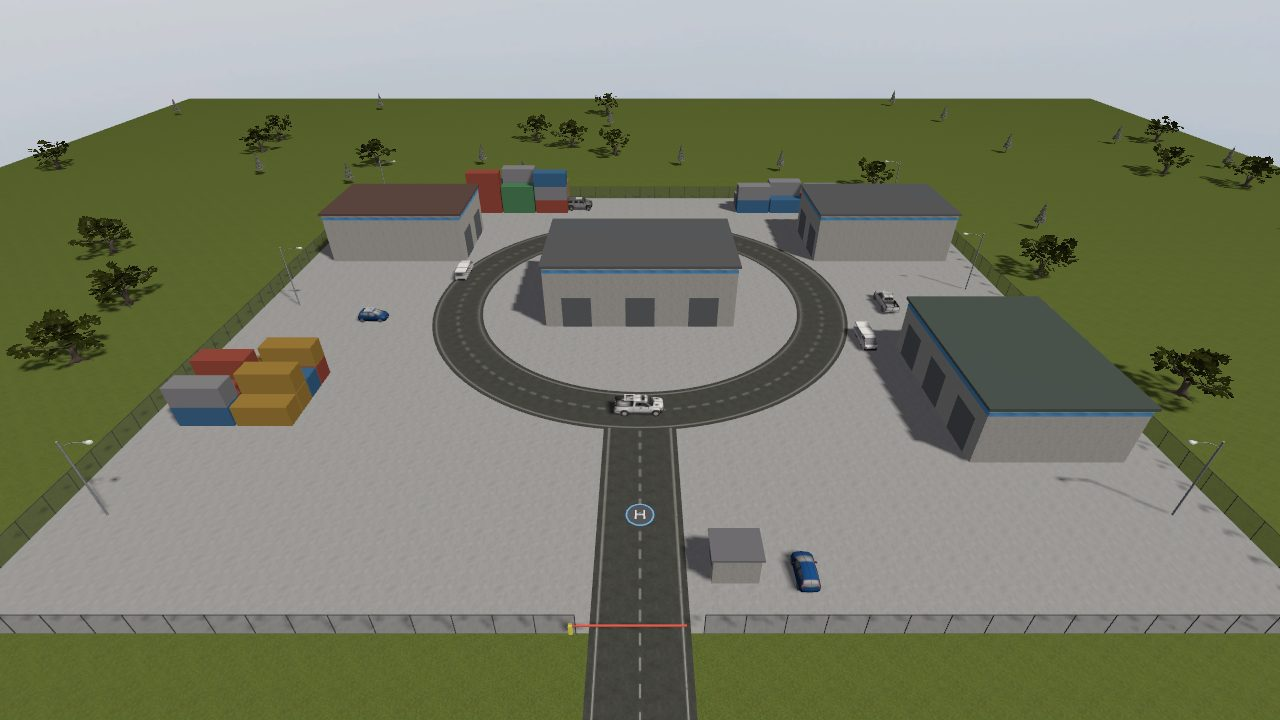
\includegraphics[width=\linewidth]{zona_bodegas}
  \end{columns}
\end{frame}

\begin{frame}[fragile]{Herramientas del paquete}
  \begin{lstlisting}[style=bash,caption={En src/x500\_retos/tools (las dos últimas con el venv del repo, trae OpenCV)}]
python3 tools/build_worlds.py                 # regenerar todos los mundos
/data/vespo_ws/venv/bin/python tools/make_aruco.py      # texturas ArUco
/data/vespo_ws/venv/bin/python tools/render_world.py plaza_show /tmp/fotos \
    "aerea:0,-36,20,0,0.5,1.5708:1.5"      # foto sin abrir Gazebo
  \end{lstlisting}
  \small \cmd{render\_world.py} agrega cámaras al mundo, corre Gazebo sin ventana con su propio
  \cmd{GZ\_PARTITION} (no choca con una simulación abierta) y guarda un PNG por cámara. Así se
  hicieron todas las capturas de esta presentación.
\end{frame}
